\documentclass[12pt,letterpaper,titlepage,en-US]{article}

\usepackage{basicstyle}
\usepackage{report}
\usepackage{knit}

\definecolor{lbcolor}{rgb}{0.969, 0.969, 0.969} 
\setlength\parindent{0pt}
 \lstset{ 
    language=C++, % choose the language of the code
    basicstyle=\fontfamily{pcr}\selectfont\footnotesize\color{black},
    keywordstyle=\color{black}, % style for keywords
    numbers=none, % where to put the line-numbers
    numberstyle=\tiny, % the size of the fonts that are used for the line-numbers     
    backgroundcolor=\color{lbcolor},
    showspaces=false, % show spaces adding particular underscores
    showstringspaces=false, % underline spaces within strings
    showtabs=false, % show tabs within strings adding particular underscores
    frame=single, % adds a frame around the code
    tabsize=2, % sets default tabsize to 2 spaces
    rulesepcolor=\color{gray},
    rulecolor=\color{black},
    captionpos=b, % sets the caption-position to bottom
    breaklines=true, % sets automatic line breaking
    breakatwhitespace=false, 
}
%
% Homework Details
%   - Title
%   - Due date
%   - Class
%   - Section/Time
%   - Instructor
%   - Author
%

\newcommand{\hmwkTitle}{Reading Assignment \#4}
\DTMsavetimestamp{DueDate}{2019-09-29T11:59:00+00:00}
\newcommand{\hmwkClass}{CS 6359.001}
\newcommand{\hmwkClassName}{Object Oriented Analysis and Design}
\newcommand{\hmwkClassInstructor}{Instructor: Prof.Mehra Nouroz Borazjany}
\newcommand{\hmwkAuthorName}{Shyam Patharla}
\newcommand{\hmwkAuthorNetID}{sxp178231}

\newcommand{\hmwkAuthorOneName}{Lizhong Zhang (lxz160730)}
\newcommand{\hmwkAuthorTwoName}{Hanlin He (hxh160630)}



%
% Title Page
%

\title{
    \vspace{1in}
    \textmd{\textbf{\hmwkClassName \\\hmwkClass:\ \hmwkTitle }}\\
    \normalsize\vspace{0.1in}\small{Due\ on\ \DTMusedate{DueDate}\ at \DTMusetime{DueDate} }\\
    \vspace{0.1in}\large{\textit{\hmwkClassInstructor}}\\
    \vspace{0.5in}
\includegraphics[height=2.4em]{UTD_logo_BW}\\
    \vspace{2in}
}

\author{\textbf{\hmwkAuthorName\ \footnotesize{(\hmwkAuthorNetID)}} \\ }
\date{}
\makeindex

\begin{document}
\maketitle


\pagenumbering{arabic}


\textbf{1. Write a brief functional description for the function.}\\
the function average() takes two parameters
\begin{itemize}[nolistsep,noitemsep]
\item \textbf{k}, an integer
\item \textbf{arr}, an array of integers
\end{itemize} 
and returns the average of the first \textbf{k} elements in the \textbf{arr} array. If the value of k is greater than the size of the list, the function returns the average of the elements in the list.\\




\textbf{2. Generate functional test cases based on functional description.}\\
In the following table we use the  variable \textbf{n} to indicate the size of the array \textbf{}.
Input: a
\begin{table}[H]
\centering
\begin{tabular}{|c|c|c|c|}
\hline
Description &Input   &Expected Output       \\\hline
Test for empty list & 	 arr of size n=0, any k 	& 0	 \\\hline
Test for single element list when $ k<1$ & arr of size n=1, k=0 & 0 \\\hline
Test for single element list &	arr of size n=1, $k>=1$	& arr[0]\\\hline
Test for $k<=n$ &  arr of size n,  $k<n$ & average of first k elements in arr \\\hline
Test for $k>n$ & arr of size n,  $k>=n$	& average of elements in arr \\\hline


\end{tabular}
\caption{Test Case Specifications}\label{1}
\end{table}


\begin{table}[H]
\centering
\begin{tabular}{|c|c|c|c|c|c|}
\hline
Description &Input   &EO & AO & Passing Criteria & Test Result    \\\hline
Test for empty list & 	 (), k=2 	& 0 & TBD & EO=AO & TBD	 \\\hline
Test for n=1 and $ k<1$ & (12), k=0 & 0 & TBD & EO=AO   & TBD \\\hline
Test for n=1 and $k>=1$ &	 (17), k=3	& 17 & TBD & EO=AO & TBD\\\hline
Test for $k<n$ &  (2, 6 ,1, 15, 20, 14), k=4  &  6 & TBD & EO=AO & TBD \\\hline
Test for $k>n$ & (2, 6, 1, 15, 20, 10), k=9 &  9 & TBD & EO=AO & TBD	  \\\hline


\end{tabular}
\caption{Tests}\label{1}
\end{table}


* EO=Expected output, AO=Actual Output, TBD=To be determined \\


\textbf{3. Identify and specify the partitions and generate partition test cases.}\\
Let L be the set of all arrays and K be the set of all possible k values.
The input domain will be \textbf{LxK} and consists of (list,k) tuples. \\

Let n = list.size()\\

Equivalence classes: 

\begin{itemize}[noitemsep,nolistsep]


\item Partition 1: Set of all (list, k) tuples where $k<n$

\item Partition 2: Set of all (list,k) tuples where $k>=n$\\
\end{itemize}
For the first set, the function average() returns the average of the first k elements in the array, while for the second set, the function returns the average of all values in the array.\\



 \textbf{4. Generate boundary value test cases.}\\
 Let \\
 nmax = maximum possible value of k\\
 nmin = minimum possible value of n \\
 kmax=max possible value of k\\
 kmin=min possible value of k\\
 
 \textbf{boundary test cases}
\begin{itemize}[noitemsep,nolistsep]


\item Partition 1: (k=nmin-1, k=nmin, k=nmin+1, k=n-1, k=n, k=n+1)
x (n=nmin-1, n=nmin,n=nmin+1, n=nmax-1, n=nmax, n=nmax+1)
\item Partition 2:  (k=n-1, k=n, k=n+1, k=nmax-1, k=nmax, k=nmax+1)
x (n=nmin-1, n=nmin,n=nmin+1, n=nmax-1, n=nmax, n=nmax+1)\\

\end{itemize}

  

  
  \textbf{5. Implement the average function in a class Average and generate test cases using Junit.} 
  
\lstinputlisting{/users/psprao/eclipse-workspace/test-driven-development/src/Average.java}
\lstinputlisting{/users/psprao/eclipse-workspace/test-driven-development/src/MyTests.java}
  

    \textbf{6.  Compile and run the test cases. Record any failures and errors that are reported. Analyze and briefly explain why each of the failures and errors occurs and how you fix them. Correct all the failures and errors until the CUT passes all the test cases. }\\
     
        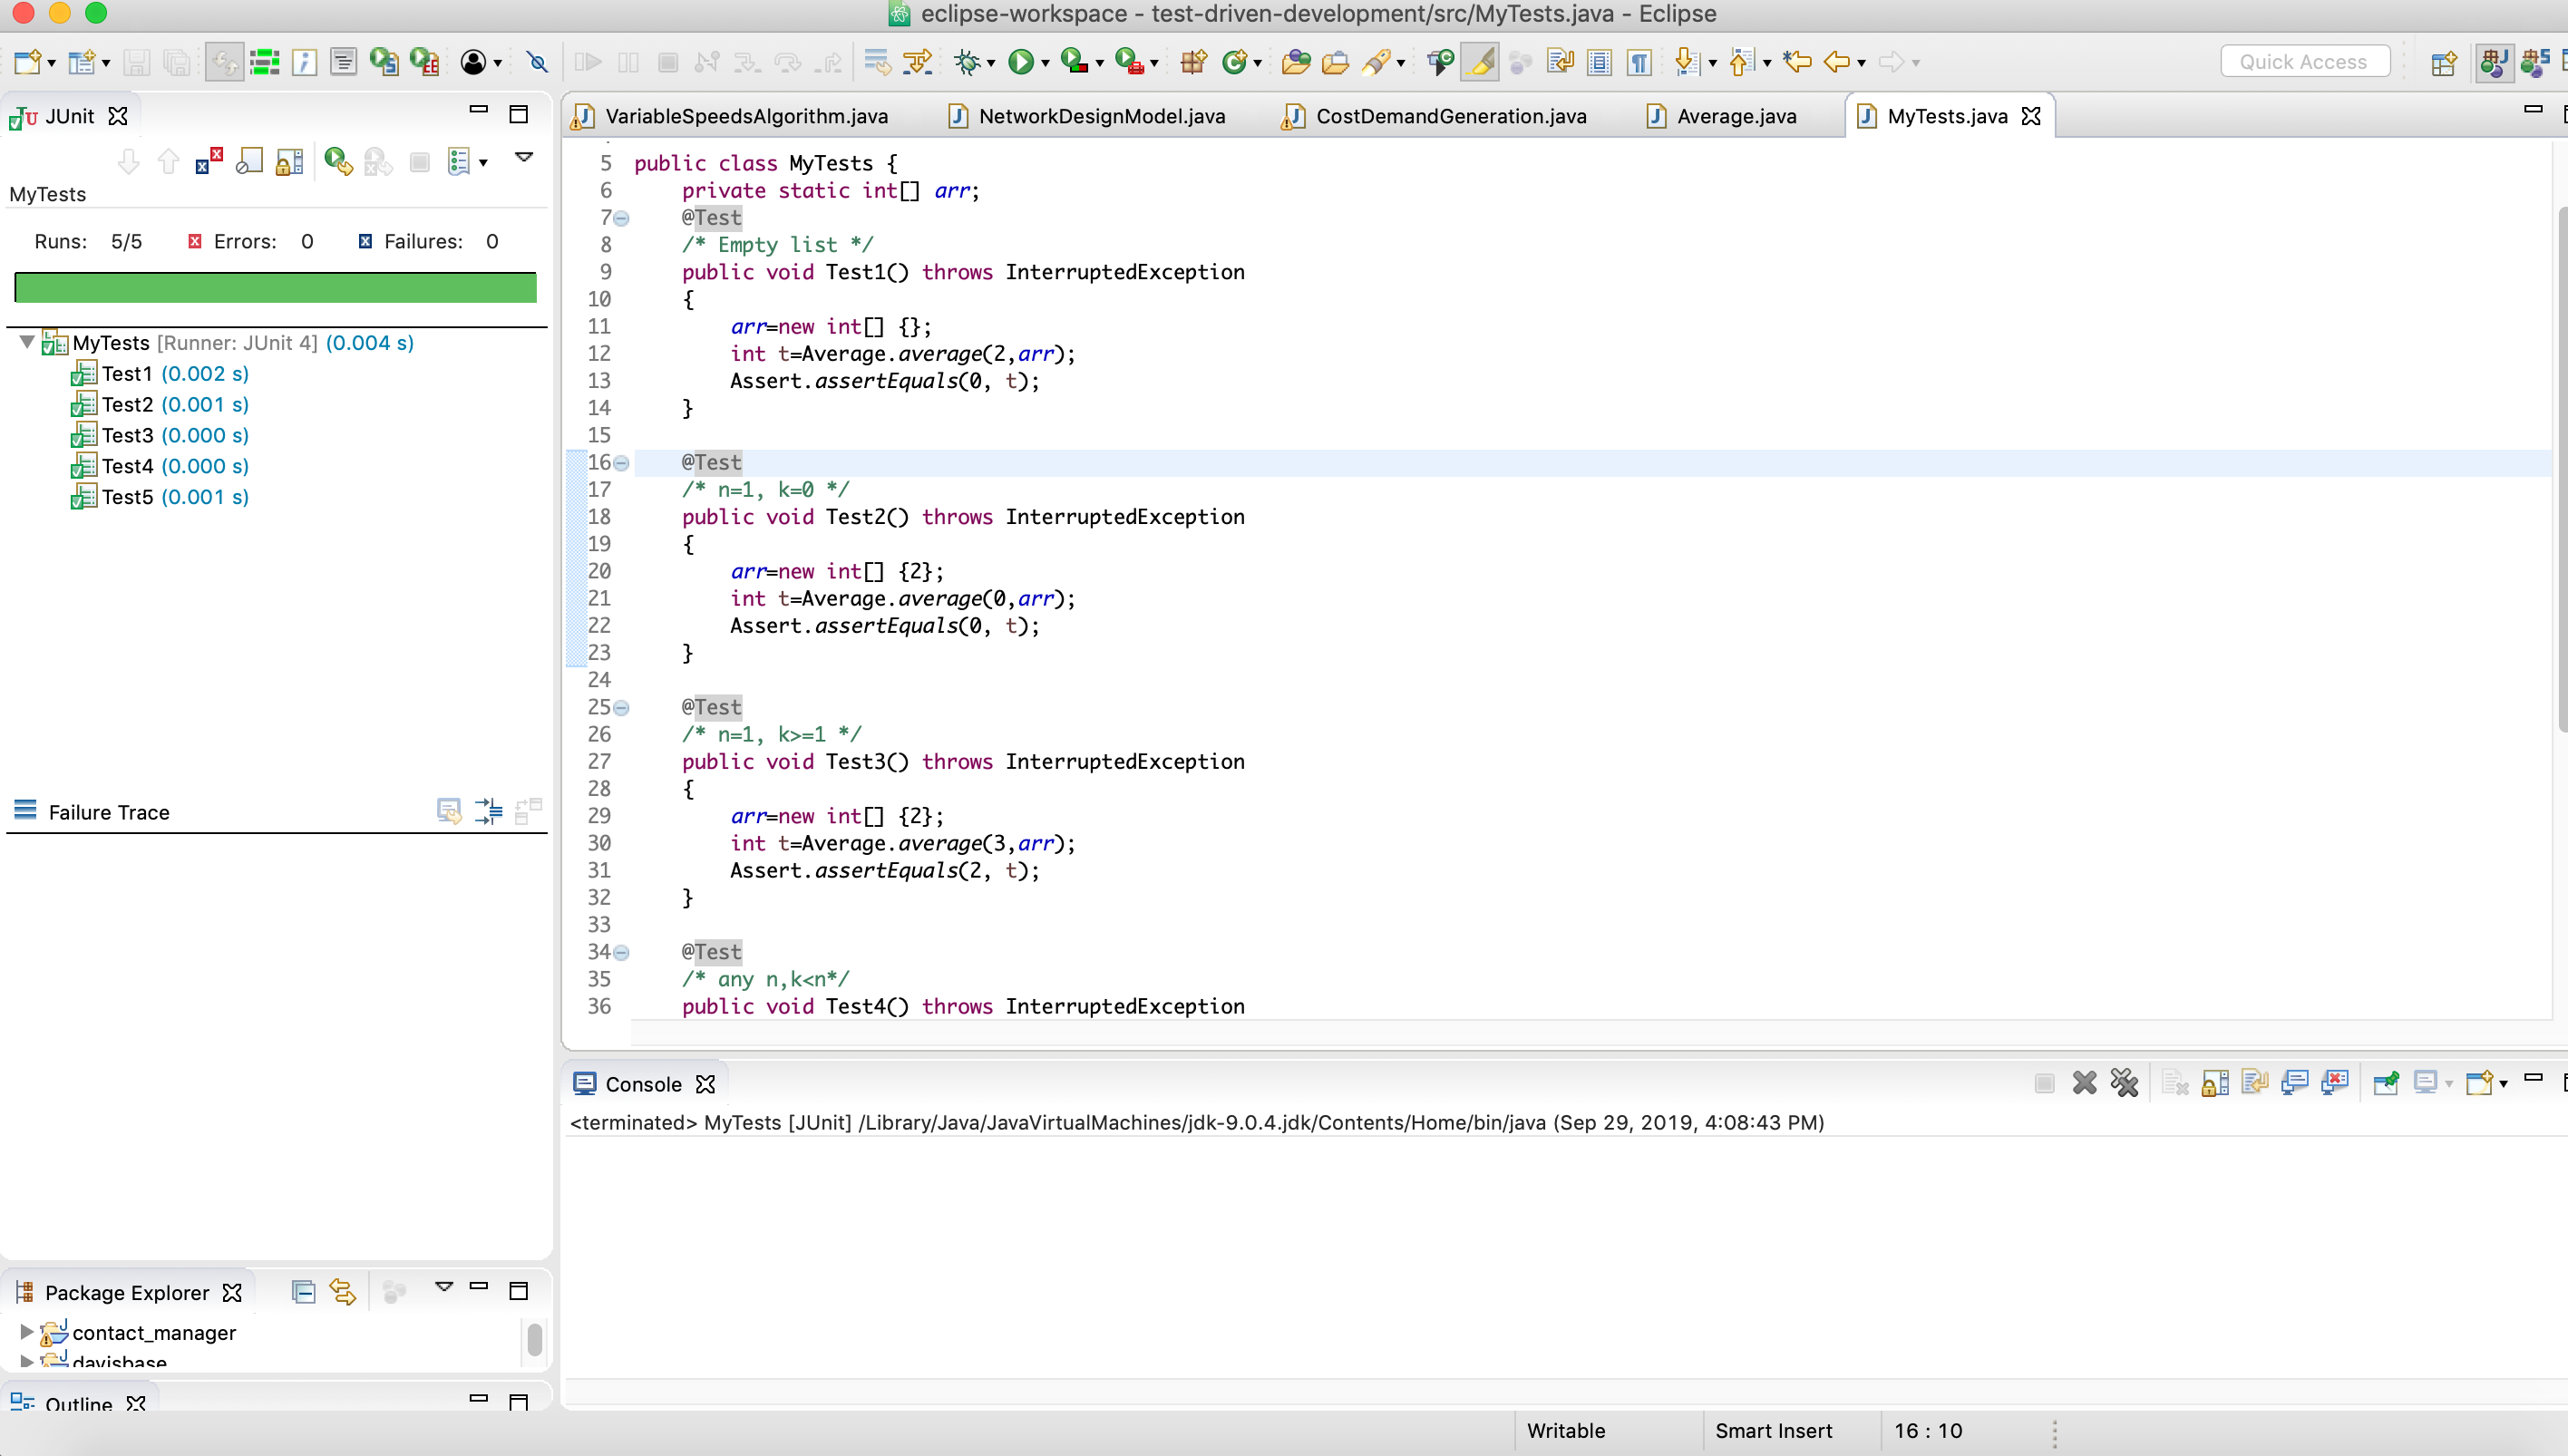
\includegraphics[scale=0.3]{testcases.png}\\
        
        
   \textbf{7. Measure the code coverage using Cobertura or other coverage tool.  }\\
We use EclEmma extension in Eclipse to measure coverage of our test cases. We get a 98\% coverage.\\
    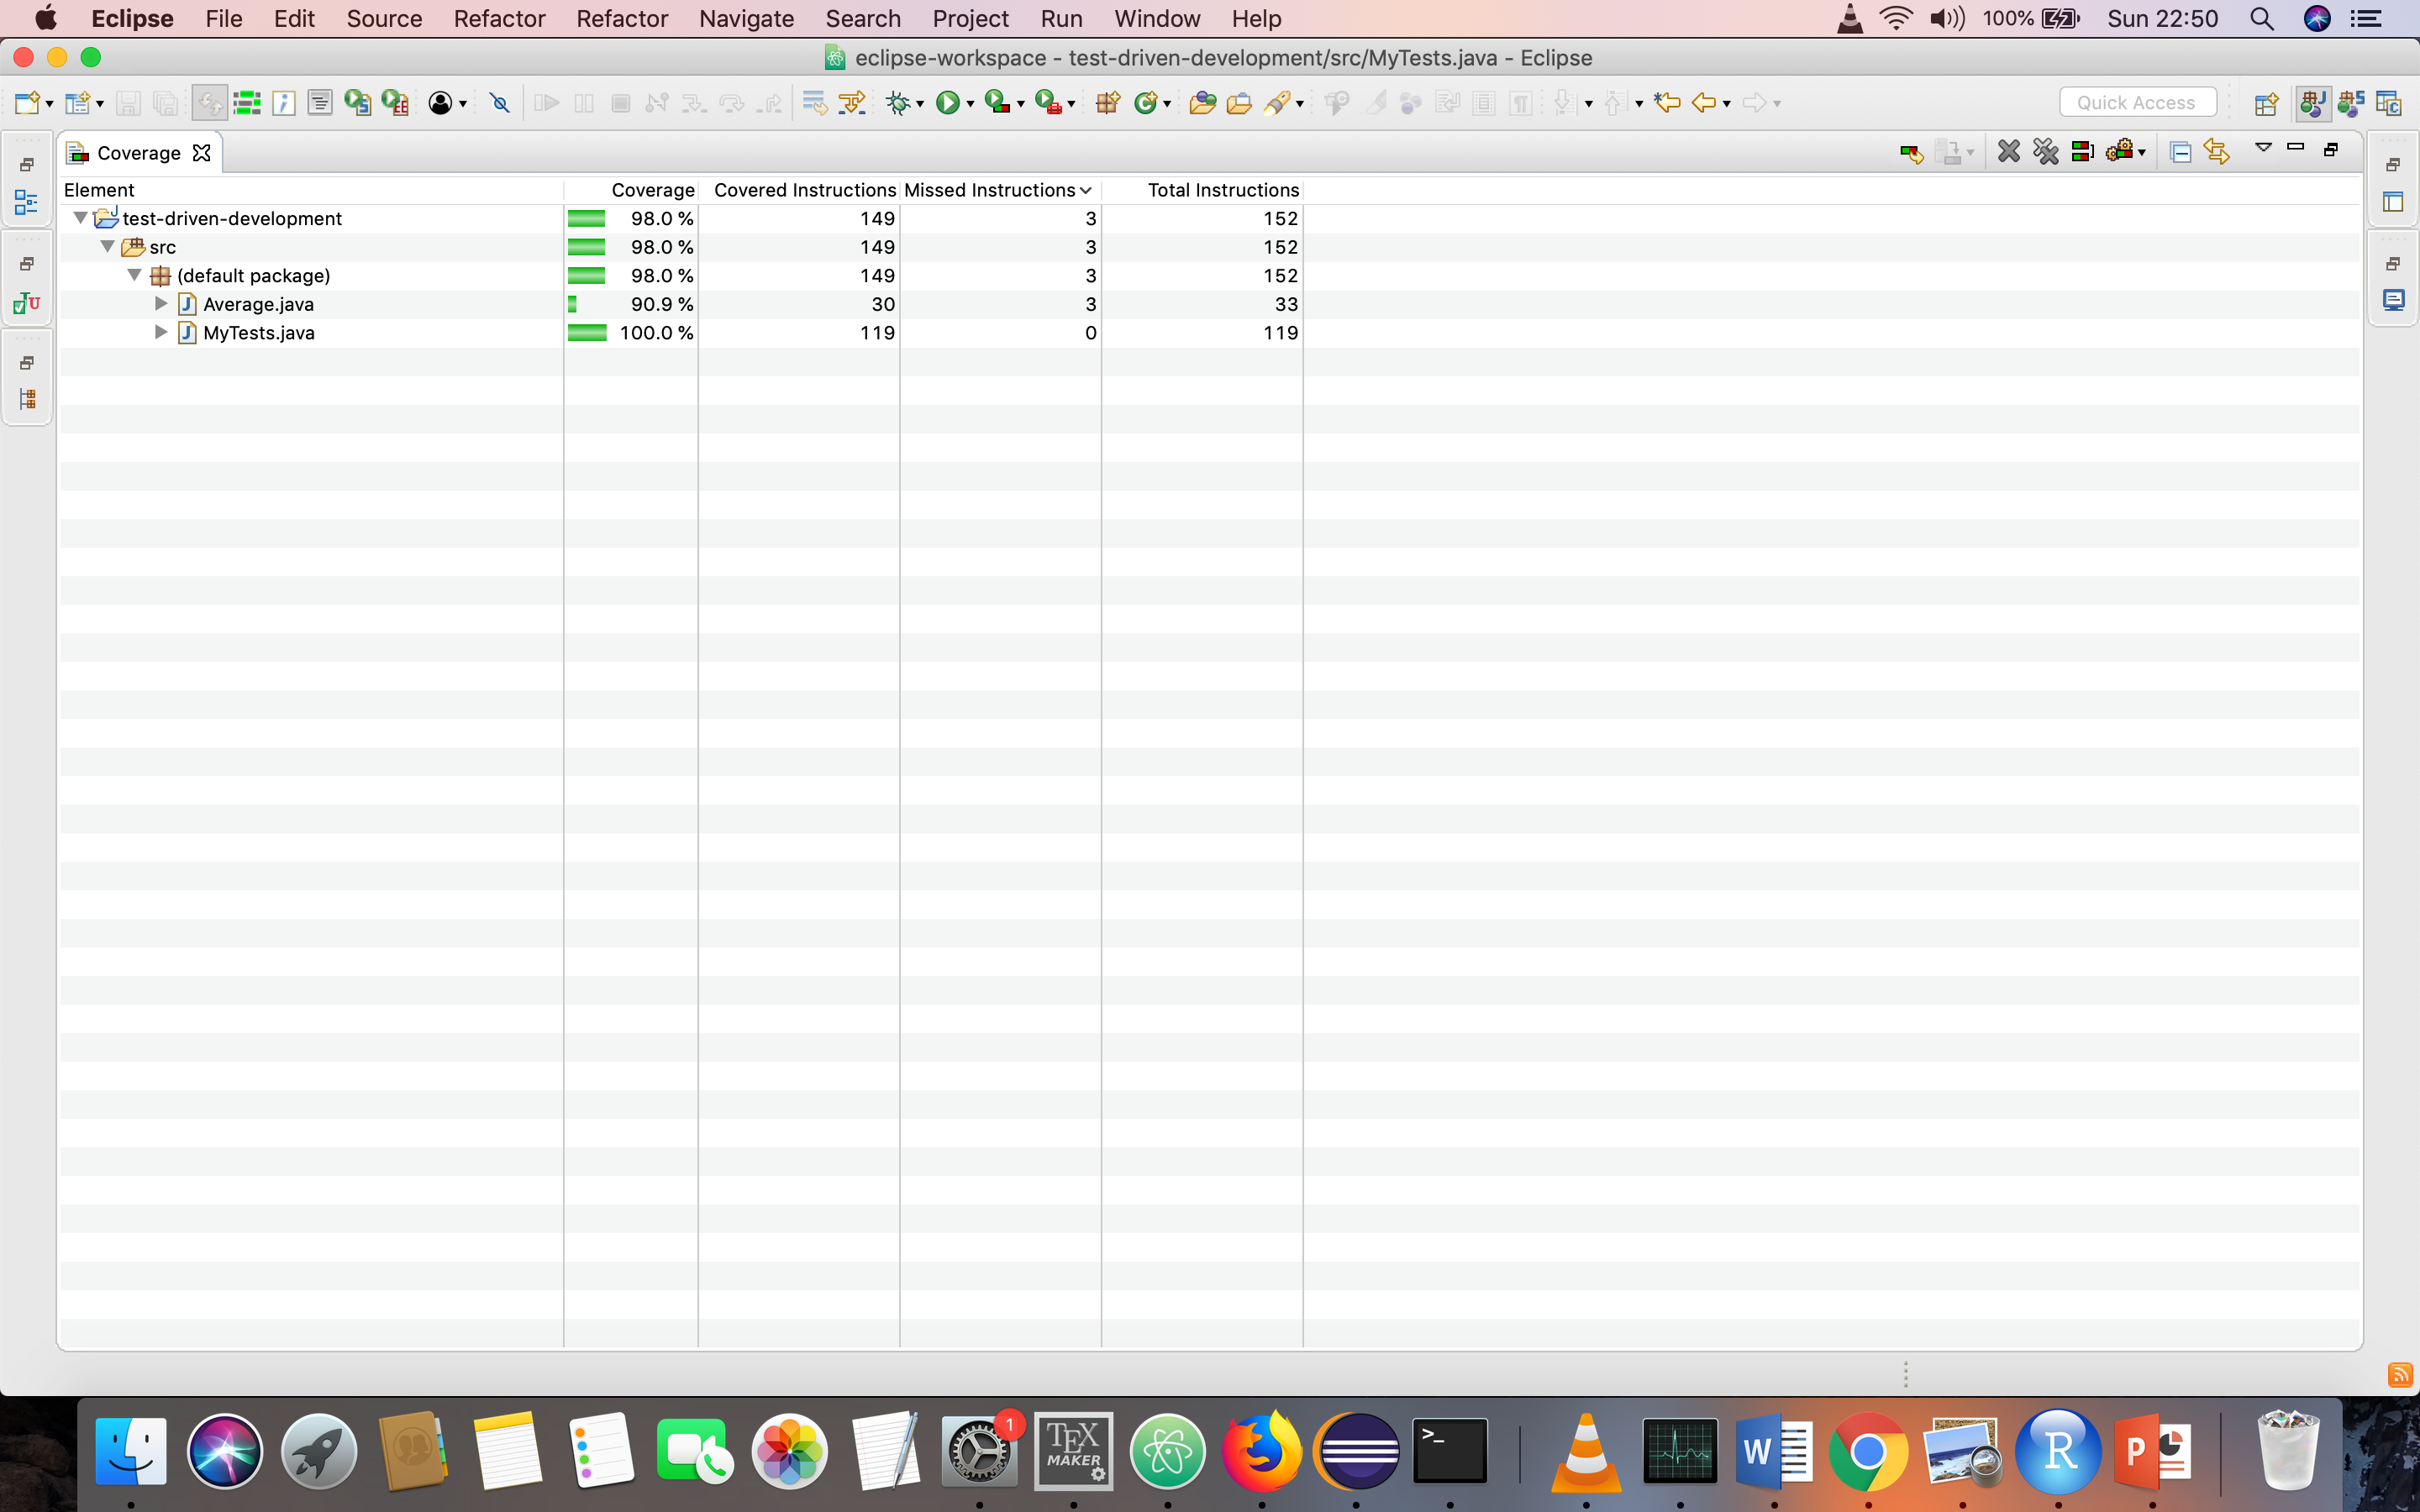
\includegraphics[scale=0.3]{coverage.png}\\
 
  


    

    
    


\textbf{Source:} Object Oriented Software Engineering: An Agile Unified Methodology, David C. Kung, McGrawHill



\end{document}
